\documentclass[1p]{elsarticle_modified}
%\bibliographystyle{elsarticle-num}

%\usepackage[colorlinks]{hyperref}
%\usepackage{abbrmath_seonhwa} %\Abb, \Ascr, \Acal ,\Abf, \Afrak
\usepackage{amsfonts}
\usepackage{amssymb}
\usepackage{amsmath}
\usepackage{amsthm}
\usepackage{scalefnt}
\usepackage{amsbsy}
\usepackage{kotex}
\usepackage{caption}
\usepackage{subfig}
\usepackage{color}
\usepackage{graphicx}
\usepackage{xcolor} %% white, black, red, green, blue, cyan, magenta, yellow
\usepackage{float}
\usepackage{setspace}
\usepackage{hyperref}

\usepackage{tikz}
\usetikzlibrary{arrows}

\usepackage{multirow}
\usepackage{array} % fixed length table
\usepackage{hhline}

%%%%%%%%%%%%%%%%%%%%%
\makeatletter
\renewcommand*\env@matrix[1][\arraystretch]{%
	\edef\arraystretch{#1}%
	\hskip -\arraycolsep
	\let\@ifnextchar\new@ifnextchar
	\array{*\c@MaxMatrixCols c}}
\makeatother %https://tex.stackexchange.com/questions/14071/how-can-i-increase-the-line-spacing-in-a-matrix
%%%%%%%%%%%%%%%

\usepackage[normalem]{ulem}

\newcommand{\msout}[1]{\ifmmode\text{\sout{\ensuremath{#1}}}\else\sout{#1}\fi}
%SOURCE: \msout is \stkout macro in https://tex.stackexchange.com/questions/20609/strikeout-in-math-mode

\newcommand{\cancel}[1]{
	\ifmmode
	{\color{red}\msout{#1}}
	\else
	{\color{red}\sout{#1}}
	\fi
}

\newcommand{\add}[1]{
	{\color{blue}\uwave{#1}}
}

\newcommand{\replace}[2]{
	\ifmmode
	{\color{red}\msout{#1}}{\color{blue}\uwave{#2}}
	\else
	{\color{red}\sout{#1}}{\color{blue}\uwave{#2}}
	\fi
}

\newcommand{\Sol}{\mathcal{S}} %segment
\newcommand{\D}{D} %diagram
\newcommand{\A}{\mathcal{A}} %arc


%%%%%%%%%%%%%%%%%%%%%%%%%%%%%5 test

\def\sl{\operatorname{\textup{SL}}(2,\Cbb)}
\def\psl{\operatorname{\textup{PSL}}(2,\Cbb)}
\def\quan{\mkern 1mu \triangleright \mkern 1mu}

\theoremstyle{definition}
\newtheorem{thm}{Theorem}[section]
\newtheorem{prop}[thm]{Proposition}
\newtheorem{lem}[thm]{Lemma}
\newtheorem{ques}[thm]{Question}
\newtheorem{cor}[thm]{Corollary}
\newtheorem{defn}[thm]{Definition}
\newtheorem{exam}[thm]{Example}
\newtheorem{rmk}[thm]{Remark}
\newtheorem{alg}[thm]{Algorithm}

\newcommand{\I}{\sqrt{-1}}
\begin{document}

%\begin{frontmatter}
%
%\title{Boundary parabolic representations of knots up to 8 crossings}
%
%%% Group authors per affiliation:
%\author{Yunhi Cho} 
%\address{Department of Mathematics, University of Seoul, Seoul, Korea}
%\ead{yhcho@uos.ac.kr}
%
%
%\author{Seonhwa Kim} %\fnref{s_kim}}
%\address{Center for Geometry and Physics, Institute for Basic Science, Pohang, 37673, Korea}
%\ead{ryeona17@ibs.re.kr}
%
%\author{Hyuk Kim}
%\address{Department of Mathematical Sciences, Seoul National University, Seoul 08826, Korea}
%\ead{hyukkim@snu.ac.kr}
%
%\author{Seokbeom Yoon}
%\address{Department of Mathematical Sciences, Seoul National University, Seoul, 08826,  Korea}
%\ead{sbyoon15@snu.ac.kr}
%
%\begin{abstract}
%We find all boundary parabolic representation of knots up to 8 crossings.
%
%\end{abstract}
%\begin{keyword}
%    \MSC[2010] 57M25 
%\end{keyword}
%
%\end{frontmatter}

%\linenumbers
%\tableofcontents
%
\newcommand\colored[1]{\textcolor{white}{\rule[-0.35ex]{0.8em}{1.4ex}}\kern-0.8em\color{red} #1}%
%\newcommand\colored[1]{\textcolor{white}{ #1}\kern-2.17ex	\textcolor{white}{ #1}\kern-1.81ex	\textcolor{white}{ #1}\kern-2.15ex\color{red}#1	}

{\Large $\underline{11n_{185}~(K11n_{185})}$}

\setlength{\tabcolsep}{10pt}
\renewcommand{\arraystretch}{1.6}
\vspace{1cm}\begin{tabular}{m{100pt}>{\centering\arraybackslash}m{274pt}}
\multirow{5}{120pt}{
	\centering
	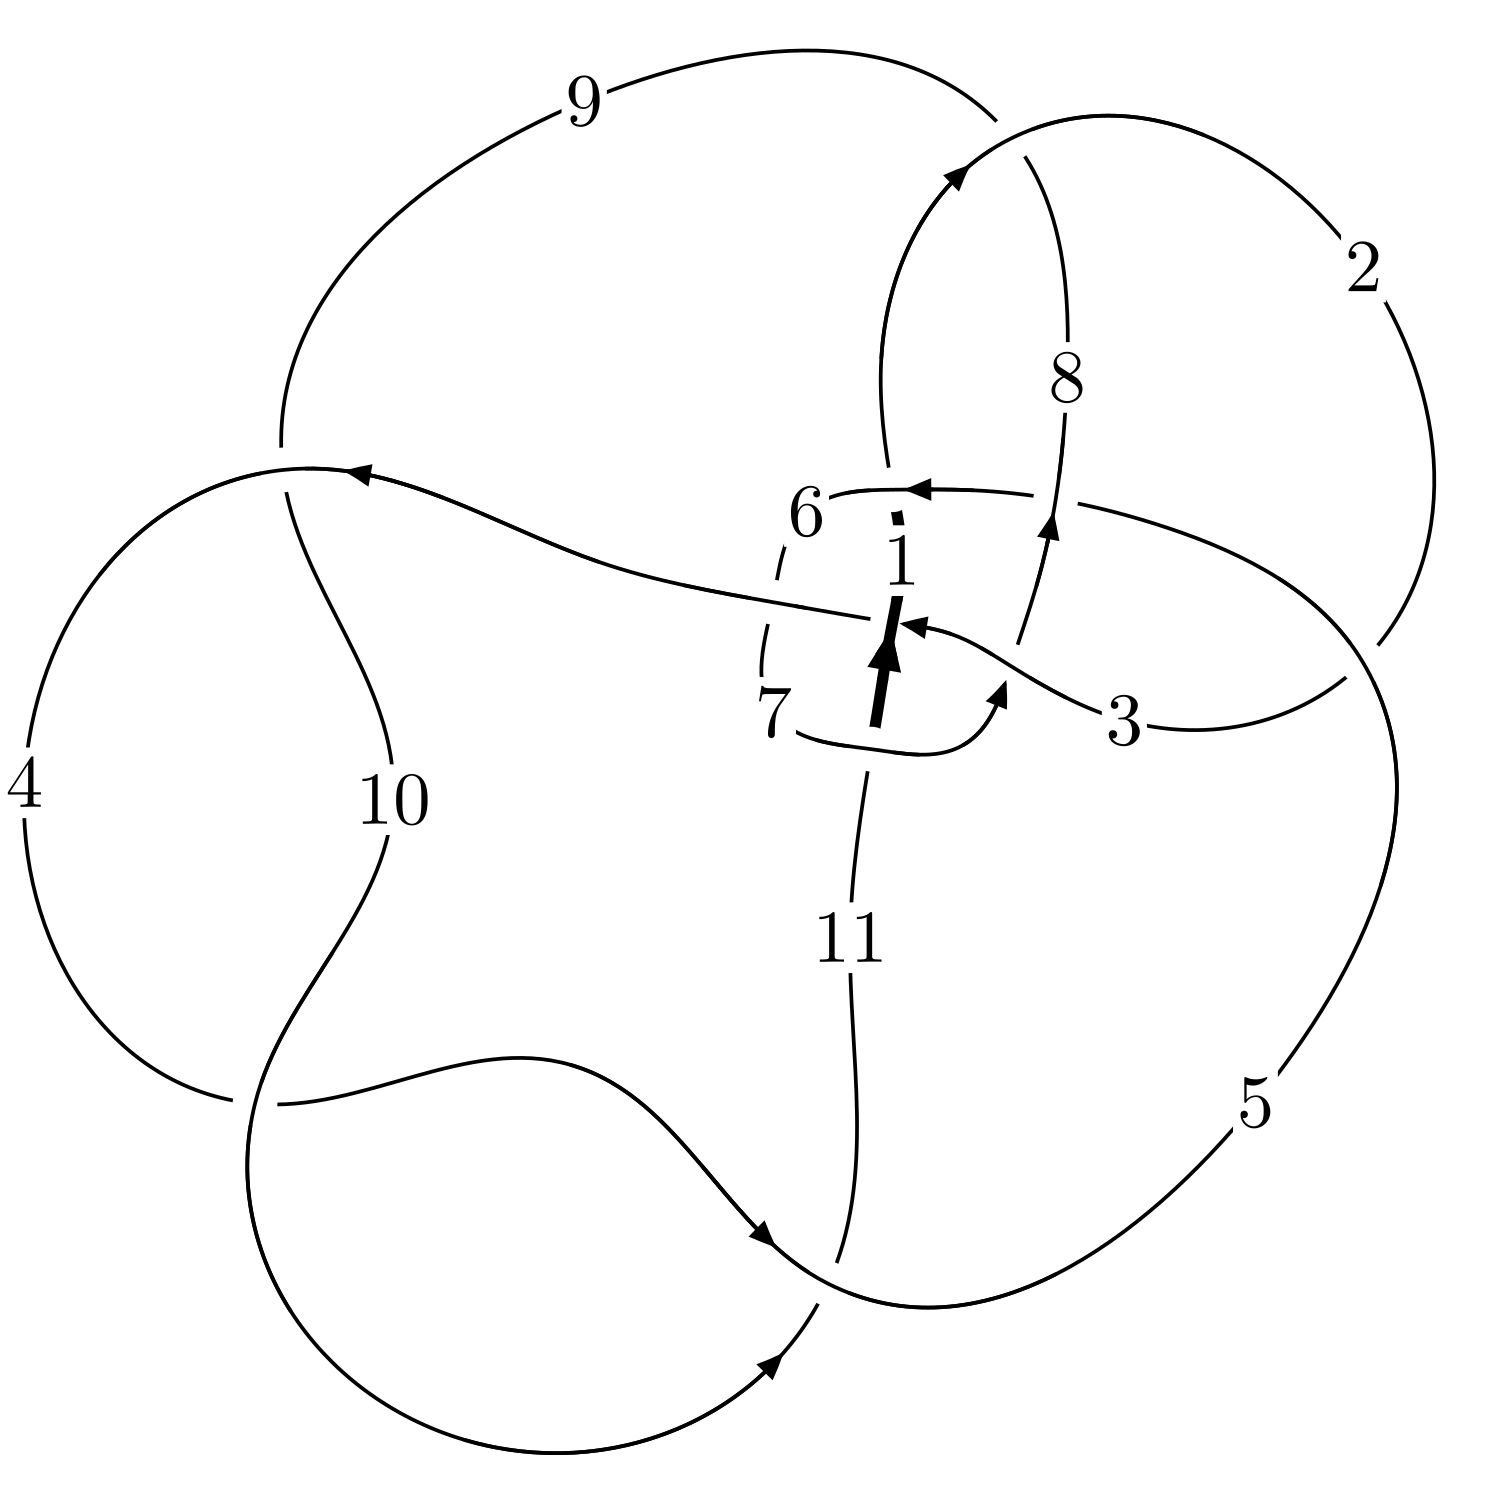
\includegraphics[width=112pt]{../../../GIT/diagram.site/Diagrams/png/801_11n_185.png}\\
\ \ \ A knot diagram\footnotemark}&
\allowdisplaybreaks
\textbf{Linearized knot diagam} \\
\cline{2-2}
 &
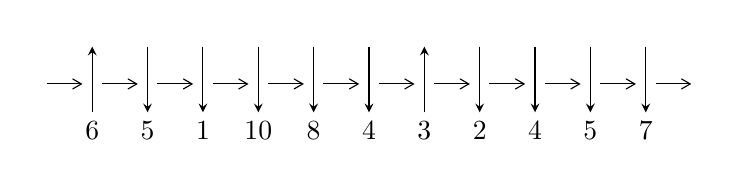
\begin{tikzpicture}[x=20pt, y=17pt]
	% nodes
	\node (C0) at (0, 0) {};
	\node (C1) at (1, 0) {};
	\node (C1U) at (1, +1) {};
	\node (C1D) at (1, -1) {6};

	\node (C2) at (2, 0) {};
	\node (C2U) at (2, +1) {};
	\node (C2D) at (2, -1) {5};

	\node (C3) at (3, 0) {};
	\node (C3U) at (3, +1) {};
	\node (C3D) at (3, -1) {1};

	\node (C4) at (4, 0) {};
	\node (C4U) at (4, +1) {};
	\node (C4D) at (4, -1) {10};

	\node (C5) at (5, 0) {};
	\node (C5U) at (5, +1) {};
	\node (C5D) at (5, -1) {8};

	\node (C6) at (6, 0) {};
	\node (C6U) at (6, +1) {};
	\node (C6D) at (6, -1) {4};

	\node (C7) at (7, 0) {};
	\node (C7U) at (7, +1) {};
	\node (C7D) at (7, -1) {3};

	\node (C8) at (8, 0) {};
	\node (C8U) at (8, +1) {};
	\node (C8D) at (8, -1) {2};

	\node (C9) at (9, 0) {};
	\node (C9U) at (9, +1) {};
	\node (C9D) at (9, -1) {4};

	\node (C10) at (10, 0) {};
	\node (C10U) at (10, +1) {};
	\node (C10D) at (10, -1) {5};

	\node (C11) at (11, 0) {};
	\node (C11U) at (11, +1) {};
	\node (C11D) at (11, -1) {7};
	\node (C12) at (12, 0) {};

	% arrows
	\draw[->,>={angle 60}]
	(C0) edge (C1) (C1) edge (C2) (C2) edge (C3) (C3) edge (C4) (C4) edge (C5) (C5) edge (C6) (C6) edge (C7) (C7) edge (C8) (C8) edge (C9) (C9) edge (C10) (C10) edge (C11) (C11) edge (C12) ;	\draw[->,>=stealth]
	(C1D) edge (C1U) (C2U) edge (C2D) (C3U) edge (C3D) (C4U) edge (C4D) (C5U) edge (C5D) (C6U) edge (C6D) (C7D) edge (C7U) (C8U) edge (C8D) (C9U) edge (C9D) (C10U) edge (C10D) (C11U) edge (C11D) ;
	\end{tikzpicture} \\
\hhline{~~} \\& 
\textbf{Solving Sequence} \\ \cline{2-2} 
 &
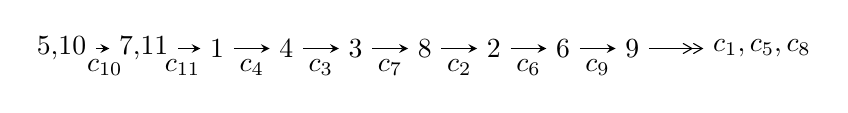
\begin{tikzpicture}[x=25pt, y=7pt]
	% node
	\node (A0) at (-1/8, 0) {5,10};
	\node (A1) at (17/16, 0) {7,11};
	\node (A2) at (17/8, 0) {1};
	\node (A3) at (25/8, 0) {4};
	\node (A4) at (33/8, 0) {3};
	\node (A5) at (41/8, 0) {8};
	\node (A6) at (49/8, 0) {2};
	\node (A7) at (57/8, 0) {6};
	\node (A8) at (65/8, 0) {9};
	\node (C1) at (1/2, -1) {$c_{10}$};
	\node (C2) at (13/8, -1) {$c_{11}$};
	\node (C3) at (21/8, -1) {$c_{4}$};
	\node (C4) at (29/8, -1) {$c_{3}$};
	\node (C5) at (37/8, -1) {$c_{7}$};
	\node (C6) at (45/8, -1) {$c_{2}$};
	\node (C7) at (53/8, -1) {$c_{6}$};
	\node (C8) at (61/8, -1) {$c_{9}$};
	\node (A9) at (10, 0) {$c_{1},c_{5},c_{8}$};

	% edge
	\draw[->,>=stealth]	
	(A0) edge (A1) (A1) edge (A2) (A2) edge (A3) (A3) edge (A4) (A4) edge (A5) (A5) edge (A6) (A6) edge (A7) (A7) edge (A8) ;
	\draw[->>,>={angle 60}]	
	(A8) edge (A9);
\end{tikzpicture} \\ 

\end{tabular} \\

\footnotetext{
The image of knot diagram is generated by the software ``\textbf{Draw programme}" developed by Andrew Bartholomew(\url{http://www.layer8.co.uk/maths/draw/index.htm\#Running-draw}), where we modified some parts for our purpose(\url{https://github.com/CATsTAILs/LinksPainter}).
}\phantom \\ \newline 
\centering \textbf{Ideals for irreducible components\footnotemark of $X_{\text{par}}$} 
 
\begin{align*}
I^u_{1}&=\langle 
-25 u^{13}-100 u^{12}+\cdots+32 b-4,\;- u^{13}+44 u^{12}+\cdots+64 a+284,\\
\phantom{I^u_{1}}&\phantom{= \langle  }u^{14}+6 u^{13}+14 u^{12}+8 u^{11}-35 u^{10}-98 u^9-105 u^8+154 u^6+224 u^5+168 u^4+74 u^3+26 u^2+16 u+8\rangle \\
I^u_{2}&=\langle 
a u+b,\;u^5 a+2 u^4 a+3 u^5+2 u^3 a+9 u^4- u^2 a+8 u^3+4 a^2- a u- u^2-10 u-7,\\
\phantom{I^u_{2}}&\phantom{= \langle  }u^6+4 u^5+6 u^4+3 u^3-3 u^2-6 u-4\rangle \\
I^u_{3}&=\langle 
-10 a^3 u^2-36 a^2 u^2+\cdots-289 a-111,\\
\phantom{I^u_{3}}&\phantom{= \langle  }a^3 u^2+a^4-2 a^3 u+3 a^2 u^2+a^3-2 a^2 u+u^2 a+3 a^2-5 a u+6 u^2+4 a-6 u+1,\;u^3- u^2+1\rangle \\
I^u_{4}&=\langle 
-2452292589 a^7 u^2+1959398184 a^6 u^2+\cdots-9164004134 a-16046840503,\\
\phantom{I^u_{4}}&\phantom{= \langle  }- a^7 u^2+10 a^6 u^2+\cdots+116 a+33,\;u^3- u^2+1\rangle \\
I^u_{5}&=\langle 
6 u^{17}+4 u^{16}+\cdots+2 b+46,\;23 u^{17}+12 u^{16}+\cdots+4 a+112,\\
\phantom{I^u_{5}}&\phantom{= \langle  }u^{18}-8 u^{16}+29 u^{14}-68 u^{12}+115 u^{10}-141 u^8+126 u^6-79 u^4+28 u^2-4\rangle \\
I^u_{6}&=\langle 
- u^2+b- u+1,\;- u^2+a+1,\;u^3+u^2-1\rangle \\
I^u_{7}&=\langle 
- a u- u^2+b+u-1,\;- u^2 a+a^2+2 a u+u^2- a+1,\;u^3- u^2+1\rangle \\
\\
I^v_{1}&=\langle 
a,\;b+1,\;v+1\rangle \\
\end{align*}
\raggedright * 8 irreducible components of $\dim_{\mathbb{C}}=0$, with total 90 representations.\\
\footnotetext{All coefficients of polynomials are rational numbers. But the coefficients are sometimes approximated in decimal forms when there is not enough margin.}
\newpage
\renewcommand{\arraystretch}{1}
\centering \section*{I. $I^u_{1}= \langle -25 u^{13}-100 u^{12}+\cdots+32 b-4,\;- u^{13}+44 u^{12}+\cdots+64 a+284,\;u^{14}+6 u^{13}+\cdots+16 u+8 \rangle$}
\flushleft \textbf{(i) Arc colorings}\\
\begin{tabular}{m{7pt} m{180pt} m{7pt} m{180pt} }
\flushright $a_{5}=$&$\begin{pmatrix}0\\u\end{pmatrix}$ \\
\flushright $a_{10}=$&$\begin{pmatrix}1\\0\end{pmatrix}$ \\
\flushright $a_{7}=$&$\begin{pmatrix}0.0156250 u^{13}-0.687500 u^{12}+\cdots-3.40625 u-4.43750\\\frac{25}{32} u^{13}+\frac{25}{8} u^{12}+\cdots+\frac{75}{16} u+\frac{1}{8}\end{pmatrix}$ \\
\flushright $a_{11}=$&$\begin{pmatrix}1\\u^2\end{pmatrix}$ \\
\flushright $a_{1}=$&$\begin{pmatrix}0.265625 u^{13}+1.56250 u^{12}+\cdots+2.59375 u+3.06250\\\frac{1}{32} u^{13}+\frac{5}{8} u^{12}+\cdots+\frac{35}{16} u+\frac{17}{8}\end{pmatrix}$ \\
\flushright $a_{4}=$&$\begin{pmatrix}u\\u\end{pmatrix}$ \\
\flushright $a_{3}=$&$\begin{pmatrix}0.765625 u^{13}+3.81250 u^{12}+\cdots+8.09375 u+4.56250\\1.34375 u^{13}+6.37500 u^{12}+\cdots+11.0625 u+6.37500\end{pmatrix}$ \\
\flushright $a_{8}=$&$\begin{pmatrix}-0.234375 u^{13}-0.937500 u^{12}+\cdots-0.406250 u-0.937500\\\frac{1}{32} u^{13}+\frac{5}{8} u^{12}+\cdots+\frac{35}{16} u+\frac{17}{8}\end{pmatrix}$ \\
\flushright $a_{2}=$&$\begin{pmatrix}0.765625 u^{13}+3.81250 u^{12}+\cdots+8.09375 u+4.56250\\\frac{25}{32} u^{13}+\frac{25}{8} u^{12}+\cdots+\frac{75}{16} u+\frac{1}{8}\end{pmatrix}$ \\
\flushright $a_{6}=$&$\begin{pmatrix}0.578125 u^{13}+2.56250 u^{12}+\cdots+2.96875 u+1.81250\\1.34375 u^{13}+6.37500 u^{12}+\cdots+11.0625 u+6.37500\end{pmatrix}$ \\
\flushright $a_{9}=$&$\begin{pmatrix}- u^2+1\\- u^2\end{pmatrix}$\\ \flushright $a_{9}=$&$\begin{pmatrix}- u^2+1\\- u^2\end{pmatrix}$\\&\end{tabular}
\flushleft \textbf{(ii) Obstruction class $= -1$}\\~\\
\flushleft \textbf{(iii) Cusp Shapes $= -\frac{11}{8} u^{13}-\frac{13}{2} u^{12}-\frac{49}{4} u^{11}-\frac{1}{2} u^{10}+\frac{361}{8} u^9+\frac{183}{2} u^8+\frac{491}{8} u^7-\frac{247}{4} u^6-\frac{673}{4} u^5-\frac{307}{2} u^4-60 u^3-\frac{23}{4} u^2-\frac{33}{4} u-\frac{31}{2}$}\\~\\
\newpage\renewcommand{\arraystretch}{1}
\flushleft \textbf{(iv) u-Polynomials at the component}\newline \\
\begin{tabular}{m{50pt}|m{274pt}}
Crossings & \hspace{64pt}u-Polynomials at each crossing \\
\hline $$\begin{aligned}c_{1},c_{7}\end{aligned}$$&$\begin{aligned}
&u^{14}- u^{13}+\cdots+2 u^2+2
\end{aligned}$\\
\hline $$\begin{aligned}c_{2},c_{6},c_{8}\\c_{11}\end{aligned}$$&$\begin{aligned}
&u^{14}- u^{13}+\cdots- u+1
\end{aligned}$\\
\hline $$\begin{aligned}c_{3},c_{5}\end{aligned}$$&$\begin{aligned}
&u^{14}-7 u^{13}+\cdots-25 u+11
\end{aligned}$\\
\hline $$\begin{aligned}c_{4},c_{9},c_{10}\end{aligned}$$&$\begin{aligned}
&u^{14}-6 u^{13}+\cdots-16 u+8
\end{aligned}$\\
\hline
\end{tabular}\\~\\
\newpage\renewcommand{\arraystretch}{1}
\flushleft \textbf{(v) Riley Polynomials at the component}\newline \\
\begin{tabular}{m{50pt}|m{274pt}}
Crossings & \hspace{64pt}Riley Polynomials at each crossing \\
\hline $$\begin{aligned}c_{1},c_{7}\end{aligned}$$&$\begin{aligned}
&y^{14}+3 y^{13}+\cdots+8 y+4
\end{aligned}$\\
\hline $$\begin{aligned}c_{2},c_{6},c_{8}\\c_{11}\end{aligned}$$&$\begin{aligned}
&y^{14}+11 y^{13}+\cdots+21 y+1
\end{aligned}$\\
\hline $$\begin{aligned}c_{3},c_{5}\end{aligned}$$&$\begin{aligned}
&y^{14}-7 y^{13}+\cdots-493 y+121
\end{aligned}$\\
\hline $$\begin{aligned}c_{4},c_{9},c_{10}\end{aligned}$$&$\begin{aligned}
&y^{14}-8 y^{13}+\cdots+160 y+64
\end{aligned}$\\
\hline
\end{tabular}\\~\\
\newpage\flushleft \textbf{(vi) Complex Volumes and Cusp Shapes}
$$\begin{array}{c|c|c}  
\text{Solutions to }I^u_{1}& \I (\text{vol} + \sqrt{-1}CS) & \text{Cusp shape}\\
 \hline 
\begin{aligned}
u &= -0.667935 + 1.025090 I \\
a &= -0.285457 - 0.894080 I \\
b &= -1.107180 - 0.304570 I\end{aligned}
 & \phantom{-}4.32333 + 2.75562 I & -3.35979 - 3.59185 I \\ \hline\begin{aligned}
u &= -0.667935 - 1.025090 I \\
a &= -0.285457 + 0.894080 I \\
b &= -1.107180 + 0.304570 I\end{aligned}
 & \phantom{-}4.32333 - 2.75562 I & -3.35979 + 3.59185 I \\ \hline\begin{aligned}
u &= -0.536682 + 1.118280 I \\
a &= \phantom{-}0.636097 + 0.907281 I \\
b &= \phantom{-}1.355980 - 0.224415 I\end{aligned}
 & \phantom{-}3.36641 - 10.30200 I & -6.23771 + 5.94221 I \\ \hline\begin{aligned}
u &= -0.536682 - 1.118280 I \\
a &= \phantom{-}0.636097 - 0.907281 I \\
b &= \phantom{-}1.355980 + 0.224415 I\end{aligned}
 & \phantom{-}3.36641 + 10.30200 I & -6.23771 - 5.94221 I \\ \hline\begin{aligned}
u &= -1.069760 + 0.720252 I \\
a &= -0.777184 - 0.841410 I \\
b &= -1.43743 - 0.34034 I\end{aligned}
 & \phantom{-}3.01100 + 3.56965 I & -5.19675 - 2.89817 I \\ \hline\begin{aligned}
u &= -1.069760 - 0.720252 I \\
a &= -0.777184 + 0.841410 I \\
b &= -1.43743 + 0.34034 I\end{aligned}
 & \phantom{-}3.01100 - 3.56965 I & -5.19675 + 2.89817 I \\ \hline\begin{aligned}
u &= -1.344910 + 0.179800 I \\
a &= \phantom{-}0.609809 - 0.501435 I \\
b &= \phantom{-}0.729978 - 0.784026 I\end{aligned}
 & -5.73092 + 3.41357 I & -11.64336 + 0.09610 I \\ \hline\begin{aligned}
u &= -1.344910 - 0.179800 I \\
a &= \phantom{-}0.609809 + 0.501435 I \\
b &= \phantom{-}0.729978 + 0.784026 I\end{aligned}
 & -5.73092 - 3.41357 I & -11.64336 - 0.09610 I \\ \hline\begin{aligned}
u &= -1.19710 + 0.78285 I \\
a &= \phantom{-}0.78383 + 1.31732 I \\
b &= \phantom{-}1.96958 + 0.96334 I\end{aligned}
 & \phantom{-}1.2941 + 17.1000 I & -8.51485 - 9.31216 I \\ \hline\begin{aligned}
u &= -1.19710 - 0.78285 I \\
a &= \phantom{-}0.78383 - 1.31732 I \\
b &= \phantom{-}1.96958 - 0.96334 I\end{aligned}
 & \phantom{-}1.2941 - 17.1000 I & -8.51485 + 9.31216 I\\
 \hline 
 \end{array}$$\newpage$$\begin{array}{c|c|c}  
\text{Solutions to }I^u_{1}& \I (\text{vol} + \sqrt{-1}CS) & \text{Cusp shape}\\
 \hline 
\begin{aligned}
u &= \phantom{-}0.252591 + 0.403462 I \\
a &= -0.828123 - 0.088481 I \\
b &= \phantom{-}0.173478 + 0.356466 I\end{aligned}
 & -0.81174 - 1.19027 I & -7.67312 + 5.52205 I \\ \hline\begin{aligned}
u &= \phantom{-}0.252591 - 0.403462 I \\
a &= -0.828123 + 0.088481 I \\
b &= \phantom{-}0.173478 - 0.356466 I\end{aligned}
 & -0.81174 + 1.19027 I & -7.67312 - 5.52205 I \\ \hline\begin{aligned}
u &= \phantom{-}1.56380 + 0.03954 I \\
a &= \phantom{-}0.111030 - 0.272749 I \\
b &= -0.184413 + 0.422135 I\end{aligned}
 & -4.62975 + 6.18029 I & -7.37442 - 7.53018 I \\ \hline\begin{aligned}
u &= \phantom{-}1.56380 - 0.03954 I \\
a &= \phantom{-}0.111030 + 0.272749 I \\
b &= -0.184413 - 0.422135 I\end{aligned}
 & -4.62975 - 6.18029 I & -7.37442 + 7.53018 I\\
 \hline 
 \end{array}$$\newpage\newpage\renewcommand{\arraystretch}{1}
\centering \section*{II. $I^u_{2}= \langle a u+b,\;u^5 a+3 u^5+\cdots+4 a^2-7,\;u^6+4 u^5+6 u^4+3 u^3-3 u^2-6 u-4 \rangle$}
\flushleft \textbf{(i) Arc colorings}\\
\begin{tabular}{m{7pt} m{180pt} m{7pt} m{180pt} }
\flushright $a_{5}=$&$\begin{pmatrix}0\\u\end{pmatrix}$ \\
\flushright $a_{10}=$&$\begin{pmatrix}1\\0\end{pmatrix}$ \\
\flushright $a_{7}=$&$\begin{pmatrix}a\\- a u\end{pmatrix}$ \\
\flushright $a_{11}=$&$\begin{pmatrix}1\\u^2\end{pmatrix}$ \\
\flushright $a_{1}=$&$\begin{pmatrix}\frac{1}{2} u^5 a-\frac{1}{4} u^5+\cdots- a+1\\u^5 a-\frac{1}{2} u^5+\cdots-2 a+1\end{pmatrix}$ \\
\flushright $a_{4}=$&$\begin{pmatrix}u\\u\end{pmatrix}$ \\
\flushright $a_{3}=$&$\begin{pmatrix}-\frac{1}{4} u^5-\frac{1}{2} u^4+\cdots+a+1\\-\frac{3}{2} u^5-3 u^4+\cdots+\frac{7}{2} u+3\end{pmatrix}$ \\
\flushright $a_{8}=$&$\begin{pmatrix}-\frac{1}{2} u^5 a+\frac{1}{4} u^5+\cdots+a-\frac{3}{2}\\- u^5 a-2 u^4 a+u^5- u^3 a+3 u^4+u^2 a+3 u^3+2 a u+2 a-2 u-3\end{pmatrix}$ \\
\flushright $a_{2}=$&$\begin{pmatrix}-\frac{1}{4} u^5-\frac{1}{2} u^4+\cdots+a+1\\-\frac{1}{2} u^5- u^4- u^3+a u+\frac{1}{2} u^2+\frac{3}{2} u+1\end{pmatrix}$ \\
\flushright $a_{6}=$&$\begin{pmatrix}- u^3 a- u^2 a+a\\- u^3 a- u^2 a- a u\end{pmatrix}$ \\
\flushright $a_{9}=$&$\begin{pmatrix}- u^2+1\\- u^2\end{pmatrix}$\\ \flushright $a_{9}=$&$\begin{pmatrix}- u^2+1\\- u^2\end{pmatrix}$\\&\end{tabular}
\flushleft \textbf{(ii) Obstruction class $= -1$}\\~\\
\flushleft \textbf{(iii) Cusp Shapes $= -14 u^5-31 u^4-31 u^3+5 u^2+28 u+30$}\\~\\
\newpage\renewcommand{\arraystretch}{1}
\flushleft \textbf{(iv) u-Polynomials at the component}\newline \\
\begin{tabular}{m{50pt}|m{274pt}}
Crossings & \hspace{64pt}u-Polynomials at each crossing \\
\hline $$\begin{aligned}c_{1},c_{7}\end{aligned}$$&$\begin{aligned}
&(u^6-2 u^4- u^3+3 u^2+u-1)^2
\end{aligned}$\\
\hline $$\begin{aligned}c_{2},c_{6},c_{8}\\c_{11}\end{aligned}$$&$\begin{aligned}
&u^{12}- u^{11}+\cdots-7 u+1
\end{aligned}$\\
\hline $$\begin{aligned}c_{3},c_{5}\end{aligned}$$&$\begin{aligned}
&u^{12}-5 u^{11}+\cdots+42 u-7
\end{aligned}$\\
\hline $$\begin{aligned}c_{4},c_{9},c_{10}\end{aligned}$$&$\begin{aligned}
&(u^6-4 u^5+6 u^4-3 u^3-3 u^2+6 u-4)^2
\end{aligned}$\\
\hline
\end{tabular}\\~\\
\newpage\renewcommand{\arraystretch}{1}
\flushleft \textbf{(v) Riley Polynomials at the component}\newline \\
\begin{tabular}{m{50pt}|m{274pt}}
Crossings & \hspace{64pt}Riley Polynomials at each crossing \\
\hline $$\begin{aligned}c_{1},c_{7}\end{aligned}$$&$\begin{aligned}
&(y^6-4 y^5+10 y^4-15 y^3+15 y^2-7 y+1)^2
\end{aligned}$\\
\hline $$\begin{aligned}c_{2},c_{6},c_{8}\\c_{11}\end{aligned}$$&$\begin{aligned}
&y^{12}+y^{11}+\cdots-59 y+1
\end{aligned}$\\
\hline $$\begin{aligned}c_{3},c_{5}\end{aligned}$$&$\begin{aligned}
&y^{12}-5 y^{11}+\cdots+154 y+49
\end{aligned}$\\
\hline $$\begin{aligned}c_{4},c_{9},c_{10}\end{aligned}$$&$\begin{aligned}
&(y^6-4 y^5+6 y^4-5 y^3-3 y^2-12 y+16)^2
\end{aligned}$\\
\hline
\end{tabular}\\~\\
\newpage\flushleft \textbf{(vi) Complex Volumes and Cusp Shapes}
$$\begin{array}{c|c|c}  
\text{Solutions to }I^u_{2}& \I (\text{vol} + \sqrt{-1}CS) & \text{Cusp shape}\\
 \hline 
\begin{aligned}
u &= \phantom{-}0.977719\phantom{ +0.000000I} \\
a &= -0.332086 + 0.227752 I \\
b &= \phantom{-}0.324687 - 0.222678 I\end{aligned}
 & -0.985708\phantom{ +0.000000I} & -7.65430\phantom{ +0.000000I} \\ \hline\begin{aligned}
u &= \phantom{-}0.977719\phantom{ +0.000000I} \\
a &= -0.332086 - 0.227752 I \\
b &= \phantom{-}0.324687 + 0.222678 I\end{aligned}
 & -0.985708\phantom{ +0.000000I} & -7.65430\phantom{ +0.000000I} \\ \hline\begin{aligned}
u &= -0.429813 + 1.015170 I \\
a &= -0.575835 - 1.071170 I \\
b &= -1.334920 + 0.124164 I\end{aligned}
 & \phantom{-}4.79788 - 2.68180 I & -2.86354 + 2.82727 I \\ \hline\begin{aligned}
u &= -0.429813 + 1.015170 I \\
a &= \phantom{-}0.024967 + 0.780798 I \\
b &= \phantom{-}0.803370 + 0.310252 I\end{aligned}
 & \phantom{-}4.79788 - 2.68180 I & -2.86354 + 2.82727 I \\ \hline\begin{aligned}
u &= -0.429813 - 1.015170 I \\
a &= -0.575835 + 1.071170 I \\
b &= -1.334920 - 0.124164 I\end{aligned}
 & \phantom{-}4.79788 + 2.68180 I & -2.86354 - 2.82727 I \\ \hline\begin{aligned}
u &= -0.429813 - 1.015170 I \\
a &= \phantom{-}0.024967 - 0.780798 I \\
b &= \phantom{-}0.803370 - 0.310252 I\end{aligned}
 & \phantom{-}4.79788 + 2.68180 I & -2.86354 - 2.82727 I \\ \hline\begin{aligned}
u &= -1.23275 + 0.71927 I \\
a &= \phantom{-}0.626848 + 0.640690 I \\
b &= \phantom{-}1.233580 + 0.338935 I\end{aligned}
 & \phantom{-}2.32551 + 9.01899 I & -7.13133 - 8.44417 I \\ \hline\begin{aligned}
u &= -1.23275 + 0.71927 I \\
a &= -0.93315 - 1.29101 I \\
b &= -2.07892 - 0.92030 I\end{aligned}
 & \phantom{-}2.32551 + 9.01899 I & -7.13133 - 8.44417 I \\ \hline\begin{aligned}
u &= -1.23275 - 0.71927 I \\
a &= \phantom{-}0.626848 - 0.640690 I \\
b &= \phantom{-}1.233580 - 0.338935 I\end{aligned}
 & \phantom{-}2.32551 - 9.01899 I & -7.13133 + 8.44417 I \\ \hline\begin{aligned}
u &= -1.23275 - 0.71927 I \\
a &= -0.93315 + 1.29101 I \\
b &= -2.07892 + 0.92030 I\end{aligned}
 & \phantom{-}2.32551 - 9.01899 I & -7.13133 + 8.44417 I\\
 \hline 
 \end{array}$$\newpage$$\begin{array}{c|c|c}  
\text{Solutions to }I^u_{2}& \I (\text{vol} + \sqrt{-1}CS) & \text{Cusp shape}\\
 \hline 
\begin{aligned}
u &= -1.65260\phantom{ +0.000000I} \\
a &= \phantom{-}1.75945\phantom{ +0.000000I} \\
b &= \phantom{-}2.90767\phantom{ +0.000000I}\end{aligned}
 & -9.97120\phantom{ +0.000000I} & \phantom{-}78.6440\phantom{ +0.000000I} \\ \hline\begin{aligned}
u &= -1.65260\phantom{ +0.000000I} \\
a &= \phantom{-}0.119054\phantom{ +0.000000I} \\
b &= \phantom{-}0.196749\phantom{ +0.000000I}\end{aligned}
 & -9.97120\phantom{ +0.000000I} & \phantom{-}78.6440\phantom{ +0.000000I}\\
 \hline 
 \end{array}$$\newpage\newpage\renewcommand{\arraystretch}{1}
\centering \section*{III. $I^u_{3}= \langle -10 a^3 u^2-36 a^2 u^2+\cdots-289 a-111,\;a^3 u^2+3 a^2 u^2+\cdots+4 a+1,\;u^3- u^2+1 \rangle$}
\flushleft \textbf{(i) Arc colorings}\\
\begin{tabular}{m{7pt} m{180pt} m{7pt} m{180pt} }
\flushright $a_{5}=$&$\begin{pmatrix}0\\u\end{pmatrix}$ \\
\flushright $a_{10}=$&$\begin{pmatrix}1\\0\end{pmatrix}$ \\
\flushright $a_{7}=$&$\begin{pmatrix}a\\0.0332226 a^{3} u^{2}+0.119601 a^{2} u^{2}+\cdots+0.960133 a+0.368771\end{pmatrix}$ \\
\flushright $a_{11}=$&$\begin{pmatrix}1\\u^2\end{pmatrix}$ \\
\flushright $a_{1}=$&$\begin{pmatrix}-0.249169 a^{3} u^{2}-0.897010 a^{2} u^{2}+\cdots-0.700997 a-0.265781\\-0.205980 a^{3} u^{2}-0.541528 a^{2} u^{2}+\cdots-0.152824 a-0.0863787\end{pmatrix}$ \\
\flushright $a_{4}=$&$\begin{pmatrix}u\\u\end{pmatrix}$ \\
\flushright $a_{3}=$&$\begin{pmatrix}-0.189369 a^{3} u^{2}-0.481728 a^{2} u^{2}+\cdots-0.172757 a-0.401993\\-0.146179 a^{3} u^{2}-0.126246 a^{2} u^{2}+\cdots+0.375415 a-0.222591\end{pmatrix}$ \\
\flushright $a_{8}=$&$\begin{pmatrix}0.0431894 a^{3} u^{2}+0.355482 a^{2} u^{2}+\cdots+0.548173 a+0.179402\\-0.176080 a^{3} u^{2}+0.166113 a^{2} u^{2}+\cdots+0.611296 a+0.345515\end{pmatrix}$ \\
\flushright $a_{2}=$&$\begin{pmatrix}-0.189369 a^{3} u^{2}-0.481728 a^{2} u^{2}+\cdots-0.172757 a-0.401993\\- a u\end{pmatrix}$ \\
\flushright $a_{6}=$&$\begin{pmatrix}0.0431894 a^{3} u^{2}+0.355482 a^{2} u^{2}+\cdots+0.548173 a+0.179402\\0.0764120 a^{3} u^{2}+0.475083 a^{2} u^{2}+\cdots+0.508306 a+0.548173\end{pmatrix}$ \\
\flushright $a_{9}=$&$\begin{pmatrix}- u^2+1\\- u^2\end{pmatrix}$\\ \flushright $a_{9}=$&$\begin{pmatrix}- u^2+1\\- u^2\end{pmatrix}$\\&\end{tabular}
\flushleft \textbf{(ii) Obstruction class $= -1$}\\~\\
\flushleft \textbf{(iii) Cusp Shapes $= -\frac{24}{301} a^3 u^2-\frac{352}{301} a^3 u-\frac{568}{301} a^2 u^2+\frac{104}{301} a^3-\frac{304}{301} a^2 u+\frac{512}{301} u^2 a+\frac{856}{301} a^2-\frac{1320}{301} a u+\frac{80}{301} u^2+\frac{992}{301} a+\frac{772}{301} u-\frac{146}{301}$}\\~\\
\newpage\renewcommand{\arraystretch}{1}
\flushleft \textbf{(iv) u-Polynomials at the component}\newline \\
\begin{tabular}{m{50pt}|m{274pt}}
Crossings & \hspace{64pt}u-Polynomials at each crossing \\
\hline $$\begin{aligned}c_{1},c_{7}\end{aligned}$$&$\begin{aligned}
&u^{12}-3 u^{11}+\cdots+30 u+25
\end{aligned}$\\
\hline $$\begin{aligned}c_{2},c_{6},c_{8}\\c_{11}\end{aligned}$$&$\begin{aligned}
&u^{12}- u^{11}+\cdots+4 u+7
\end{aligned}$\\
\hline $$\begin{aligned}c_{3},c_{5}\end{aligned}$$&$\begin{aligned}
&(u^2+u+1)^6
\end{aligned}$\\
\hline $$\begin{aligned}c_{4},c_{9},c_{10}\end{aligned}$$&$\begin{aligned}
&(u^3+u^2-1)^4
\end{aligned}$\\
\hline
\end{tabular}\\~\\
\newpage\renewcommand{\arraystretch}{1}
\flushleft \textbf{(v) Riley Polynomials at the component}\newline \\
\begin{tabular}{m{50pt}|m{274pt}}
Crossings & \hspace{64pt}Riley Polynomials at each crossing \\
\hline $$\begin{aligned}c_{1},c_{7}\end{aligned}$$&$\begin{aligned}
&y^{12}-9 y^{11}+\cdots-100 y+625
\end{aligned}$\\
\hline $$\begin{aligned}c_{2},c_{6},c_{8}\\c_{11}\end{aligned}$$&$\begin{aligned}
&y^{12}+3 y^{11}+\cdots+208 y+49
\end{aligned}$\\
\hline $$\begin{aligned}c_{3},c_{5}\end{aligned}$$&$\begin{aligned}
&(y^2+y+1)^6
\end{aligned}$\\
\hline $$\begin{aligned}c_{4},c_{9},c_{10}\end{aligned}$$&$\begin{aligned}
&(y^3- y^2+2 y-1)^4
\end{aligned}$\\
\hline
\end{tabular}\\~\\
\newpage\flushleft \textbf{(vi) Complex Volumes and Cusp Shapes}
$$\begin{array}{c|c|c}  
\text{Solutions to }I^u_{3}& \I (\text{vol} + \sqrt{-1}CS) & \text{Cusp shape}\\
 \hline 
\begin{aligned}
u &= \phantom{-}0.877439 + 0.744862 I \\
a &= \phantom{-}1.163500 - 0.426968 I \\
b &= \phantom{-}1.65706 - 0.08153 I\end{aligned}
 & \phantom{-}3.02413 + 1.23164 I & -2.49024 - 3.94876 I \\ \hline\begin{aligned}
u &= \phantom{-}0.877439 + 0.744862 I \\
a &= -0.014457 + 1.385720 I \\
b &= -1.70063 + 1.21638 I\end{aligned}
 & \phantom{-}3.02413 - 6.88789 I & -2.49024 + 9.90765 I \\ \hline\begin{aligned}
u &= \phantom{-}0.877439 + 0.744862 I \\
a &= -1.05173 + 0.98574 I \\
b &= -1.33894 - 0.49201 I\end{aligned}
 & \phantom{-}3.02413 + 1.23164 I & -2.49024 - 3.94876 I \\ \hline\begin{aligned}
u &= \phantom{-}0.877439 + 0.744862 I \\
a &= \phantom{-}0.44248 - 1.76191 I \\
b &= \phantom{-}1.04486 - 1.20512 I\end{aligned}
 & \phantom{-}3.02413 - 6.88789 I & -2.49024 + 9.90765 I \\ \hline\begin{aligned}
u &= \phantom{-}0.877439 - 0.744862 I \\
a &= \phantom{-}1.163500 + 0.426968 I \\
b &= \phantom{-}1.65706 + 0.08153 I\end{aligned}
 & \phantom{-}3.02413 - 1.23164 I & -2.49024 + 3.94876 I \\ \hline\begin{aligned}
u &= \phantom{-}0.877439 - 0.744862 I \\
a &= -0.014457 - 1.385720 I \\
b &= -1.70063 - 1.21638 I\end{aligned}
 & \phantom{-}3.02413 + 6.88789 I & -2.49024 - 9.90765 I \\ \hline\begin{aligned}
u &= \phantom{-}0.877439 - 0.744862 I \\
a &= -1.05173 - 0.98574 I \\
b &= -1.33894 + 0.49201 I\end{aligned}
 & \phantom{-}3.02413 - 1.23164 I & -2.49024 + 3.94876 I \\ \hline\begin{aligned}
u &= \phantom{-}0.877439 - 0.744862 I \\
a &= \phantom{-}0.44248 + 1.76191 I \\
b &= \phantom{-}1.04486 + 1.20512 I\end{aligned}
 & \phantom{-}3.02413 + 6.88789 I & -2.49024 - 9.90765 I \\ \hline\begin{aligned}
u &= -0.754878\phantom{ +0.000000I} \\
a &= -0.03389 + 1.64154 I \\
b &= -1.136780 + 0.774104 I\end{aligned}
 & -1.11345 - 4.05977 I & -9.01951 + 6.92820 I \\ \hline\begin{aligned}
u &= -0.754878\phantom{ +0.000000I} \\
a &= -0.03389 - 1.64154 I \\
b &= -1.136780 - 0.774104 I\end{aligned}
 & -1.11345 + 4.05977 I & -9.01951 - 6.92820 I\\
 \hline 
 \end{array}$$\newpage$$\begin{array}{c|c|c}  
\text{Solutions to }I^u_{3}& \I (\text{vol} + \sqrt{-1}CS) & \text{Cusp shape}\\
 \hline 
\begin{aligned}
u &= -0.754878\phantom{ +0.000000I} \\
a &= -1.50591 + 1.02547 I \\
b &= -0.025581 + 1.239160 I\end{aligned}
 & -1.11345 - 4.05977 I & -9.01951 + 6.92820 I \\ \hline\begin{aligned}
u &= -0.754878\phantom{ +0.000000I} \\
a &= -1.50591 - 1.02547 I \\
b &= -0.025581 - 1.239160 I\end{aligned}
 & -1.11345 + 4.05977 I & -9.01951 - 6.92820 I\\
 \hline 
 \end{array}$$\newpage\newpage\renewcommand{\arraystretch}{1}
\centering \section*{IV. $I^u_{4}= \langle -2.45\times10^{9} a^{7} u^{2}+1.96\times10^{9} a^{6} u^{2}+\cdots-9.16\times10^{9} a-1.60\times10^{10},\;- a^7 u^2+10 a^6 u^2+\cdots+116 a+33,\;u^3- u^2+1 \rangle$}
\flushleft \textbf{(i) Arc colorings}\\
\begin{tabular}{m{7pt} m{180pt} m{7pt} m{180pt} }
\flushright $a_{5}=$&$\begin{pmatrix}0\\u\end{pmatrix}$ \\
\flushright $a_{10}=$&$\begin{pmatrix}1\\0\end{pmatrix}$ \\
\flushright $a_{7}=$&$\begin{pmatrix}a\\0.405041 a^{7} u^{2}-0.323630 a^{6} u^{2}+\cdots+1.51360 a+2.65043\end{pmatrix}$ \\
\flushright $a_{11}=$&$\begin{pmatrix}1\\u^2\end{pmatrix}$ \\
\flushright $a_{1}=$&$\begin{pmatrix}-0.523501 a^{7} u^{2}-0.0850496 a^{6} u^{2}+\cdots-0.741341 a-0.113356\\-0.280191 a^{7} u^{2}-0.209408 a^{6} u^{2}+\cdots+2.44721 a+3.96214\end{pmatrix}$ \\
\flushright $a_{4}=$&$\begin{pmatrix}u\\u\end{pmatrix}$ \\
\flushright $a_{3}=$&$\begin{pmatrix}-0.0502811 a^{7} u^{2}-0.392110 a^{6} u^{2}+\cdots+1.40914 a+0.793861\\-0.124389 a^{7} u^{2}-0.527176 a^{6} u^{2}+\cdots+9.80960 a+8.21031\end{pmatrix}$ \\
\flushright $a_{8}=$&$\begin{pmatrix}-0.232267 a^{7} u^{2}+0.0446991 a^{6} u^{2}+\cdots+0.0658781 a-1.11663\\0.338024 a^{7} u^{2}+0.201586 a^{6} u^{2}+\cdots+2.61051 a-0.410883\end{pmatrix}$ \\
\flushright $a_{2}=$&$\begin{pmatrix}-0.0502811 a^{7} u^{2}-0.392110 a^{6} u^{2}+\cdots+1.40914 a+0.793861\\0.342964 a^{7} u^{2}-0.298685 a^{6} u^{2}+\cdots+10.1678 a+8.72007\end{pmatrix}$ \\
\flushright $a_{6}=$&$\begin{pmatrix}0.107236 a^{7} u^{2}-0.103911 a^{6} u^{2}+\cdots+1.36281 a+1.46016\\0.512277 a^{7} u^{2}-0.427541 a^{6} u^{2}+\cdots+1.87642 a+4.11059\end{pmatrix}$ \\
\flushright $a_{9}=$&$\begin{pmatrix}- u^2+1\\- u^2\end{pmatrix}$\\ \flushright $a_{9}=$&$\begin{pmatrix}- u^2+1\\- u^2\end{pmatrix}$\\&\end{tabular}
\flushleft \textbf{(ii) Obstruction class $= -1$}\\~\\
\flushleft \textbf{(iii) Cusp Shapes $= \frac{8159408}{12909239} a^7 u^2-\frac{2809816}{1844177} a^6 u^2+\cdots+\frac{257953072}{12909239} a-\frac{2299186}{12909239}$}\\~\\
\newpage\renewcommand{\arraystretch}{1}
\flushleft \textbf{(iv) u-Polynomials at the component}\newline \\
\begin{tabular}{m{50pt}|m{274pt}}
Crossings & \hspace{64pt}u-Polynomials at each crossing \\
\hline $$\begin{aligned}c_{1},c_{7}\end{aligned}$$&$\begin{aligned}
&(u^{12}+u^{11}+\cdots-4 u+1)^{2}
\end{aligned}$\\
\hline $$\begin{aligned}c_{2},c_{6},c_{8}\\c_{11}\end{aligned}$$&$\begin{aligned}
&u^{24}+u^{23}+\cdots+94 u+19
\end{aligned}$\\
\hline $$\begin{aligned}c_{3},c_{5}\end{aligned}$$&$\begin{aligned}
&(u^4+u^3-2 u+1)^6
\end{aligned}$\\
\hline $$\begin{aligned}c_{4},c_{9},c_{10}\end{aligned}$$&$\begin{aligned}
&(u^3+u^2-1)^8
\end{aligned}$\\
\hline
\end{tabular}\\~\\
\newpage\renewcommand{\arraystretch}{1}
\flushleft \textbf{(v) Riley Polynomials at the component}\newline \\
\begin{tabular}{m{50pt}|m{274pt}}
Crossings & \hspace{64pt}Riley Polynomials at each crossing \\
\hline $$\begin{aligned}c_{1},c_{7}\end{aligned}$$&$\begin{aligned}
&(y^{12}+3 y^{11}+\cdots-8 y+1)^{2}
\end{aligned}$\\
\hline $$\begin{aligned}c_{2},c_{6},c_{8}\\c_{11}\end{aligned}$$&$\begin{aligned}
&y^{24}-15 y^{23}+\cdots+6136 y+361
\end{aligned}$\\
\hline $$\begin{aligned}c_{3},c_{5}\end{aligned}$$&$\begin{aligned}
&(y^4- y^3+6 y^2-4 y+1)^6
\end{aligned}$\\
\hline $$\begin{aligned}c_{4},c_{9},c_{10}\end{aligned}$$&$\begin{aligned}
&(y^3- y^2+2 y-1)^8
\end{aligned}$\\
\hline
\end{tabular}\\~\\
\newpage\flushleft \textbf{(vi) Complex Volumes and Cusp Shapes}
$$\begin{array}{c|c|c}  
\text{Solutions to }I^u_{4}& \I (\text{vol} + \sqrt{-1}CS) & \text{Cusp shape}\\
 \hline 
\begin{aligned}
u &= \phantom{-}0.877439 + 0.744862 I \\
a &= -0.781244 - 0.526293 I \\
b &= -1.57291 - 0.16189 I\end{aligned}
 & -0.26574 - 6.88789 I & -14.4902 + 9.9077 I \\ \hline\begin{aligned}
u &= \phantom{-}0.877439 + 0.744862 I \\
a &= -0.931824 + 0.522997 I \\
b &= -0.957160 - 0.116334 I\end{aligned}
 & -0.265740 + 1.231640 I & -14.4902 - 3.9488 I \\ \hline\begin{aligned}
u &= \phantom{-}0.877439 + 0.744862 I \\
a &= \phantom{-}0.699396 - 0.461137 I \\
b &= \phantom{-}1.207180 + 0.235183 I\end{aligned}
 & -0.265740 + 1.231640 I & -14.4902 - 3.9488 I \\ \hline\begin{aligned}
u &= \phantom{-}0.877439 + 0.744862 I \\
a &= -0.065722 + 1.213540 I \\
b &= \phantom{-}0.418059 + 0.300929 I\end{aligned}
 & -0.265740 + 1.231640 I & -14.4902 - 3.9488 I \\ \hline\begin{aligned}
u &= \phantom{-}0.877439 + 0.744862 I \\
a &= \phantom{-}1.132860 - 0.777183 I \\
b &= \phantom{-}0.293478 + 1.043710 I\end{aligned}
 & -0.26574 - 6.88789 I & -14.4902 + 9.9077 I \\ \hline\begin{aligned}
u &= \phantom{-}0.877439 + 0.744862 I \\
a &= -0.222091 + 1.383150 I \\
b &= -1.23772 + 1.32475 I\end{aligned}
 & -0.26574 - 6.88789 I & -14.4902 + 9.9077 I \\ \hline\begin{aligned}
u &= \phantom{-}0.877439 + 0.744862 I \\
a &= -0.446111 + 0.035743 I \\
b &= \phantom{-}0.961588 - 1.015860 I\end{aligned}
 & -0.265740 + 1.231640 I & -14.4902 - 3.9488 I \\ \hline\begin{aligned}
u &= \phantom{-}0.877439 + 0.744862 I \\
a &= \phantom{-}0.07494 - 1.57340 I \\
b &= \phantom{-}1.22513 - 1.04820 I\end{aligned}
 & -0.26574 - 6.88789 I & -14.4902 + 9.9077 I \\ \hline\begin{aligned}
u &= \phantom{-}0.877439 - 0.744862 I \\
a &= -0.781244 + 0.526293 I \\
b &= -1.57291 + 0.16189 I\end{aligned}
 & -0.26574 + 6.88789 I & -14.4902 - 9.9077 I \\ \hline\begin{aligned}
u &= \phantom{-}0.877439 - 0.744862 I \\
a &= -0.931824 - 0.522997 I \\
b &= -0.957160 + 0.116334 I\end{aligned}
 & -0.265740 - 1.231640 I & -14.4902 + 3.9488 I\\
 \hline 
 \end{array}$$\newpage$$\begin{array}{c|c|c}  
\text{Solutions to }I^u_{4}& \I (\text{vol} + \sqrt{-1}CS) & \text{Cusp shape}\\
 \hline 
\begin{aligned}
u &= \phantom{-}0.877439 - 0.744862 I \\
a &= \phantom{-}0.699396 + 0.461137 I \\
b &= \phantom{-}1.207180 - 0.235183 I\end{aligned}
 & -0.265740 - 1.231640 I & -14.4902 + 3.9488 I \\ \hline\begin{aligned}
u &= \phantom{-}0.877439 - 0.744862 I \\
a &= -0.065722 - 1.213540 I \\
b &= \phantom{-}0.418059 - 0.300929 I\end{aligned}
 & -0.265740 - 1.231640 I & -14.4902 + 3.9488 I \\ \hline\begin{aligned}
u &= \phantom{-}0.877439 - 0.744862 I \\
a &= \phantom{-}1.132860 + 0.777183 I \\
b &= \phantom{-}0.293478 - 1.043710 I\end{aligned}
 & -0.26574 + 6.88789 I & -14.4902 - 9.9077 I \\ \hline\begin{aligned}
u &= \phantom{-}0.877439 - 0.744862 I \\
a &= -0.222091 - 1.383150 I \\
b &= -1.23772 - 1.32475 I\end{aligned}
 & -0.26574 + 6.88789 I & -14.4902 - 9.9077 I \\ \hline\begin{aligned}
u &= \phantom{-}0.877439 - 0.744862 I \\
a &= -0.446111 - 0.035743 I \\
b &= \phantom{-}0.961588 + 1.015860 I\end{aligned}
 & -0.265740 - 1.231640 I & -14.4902 + 3.9488 I \\ \hline\begin{aligned}
u &= \phantom{-}0.877439 - 0.744862 I \\
a &= \phantom{-}0.07494 + 1.57340 I \\
b &= \phantom{-}1.22513 + 1.04820 I\end{aligned}
 & -0.26574 + 6.88789 I & -14.4902 - 9.9077 I \\ \hline\begin{aligned}
u &= -0.754878\phantom{ +0.000000I} \\
a &= -0.421556 + 0.043844 I \\
b &= \phantom{-}1.135590 + 0.509778 I\end{aligned}
 & -4.40332 - 4.05977 I & -21.0195 + 6.9282 I \\ \hline\begin{aligned}
u &= -0.754878\phantom{ +0.000000I} \\
a &= -0.421556 - 0.043844 I \\
b &= \phantom{-}1.135590 - 0.509778 I\end{aligned}
 & -4.40332 + 4.05977 I & -21.0195 - 6.9282 I \\ \hline\begin{aligned}
u &= -0.754878\phantom{ +0.000000I} \\
a &= \phantom{-}1.50433 + 0.67531 I \\
b &= -0.318223 + 0.033097 I\end{aligned}
 & -4.40332 - 4.05977 I & -21.0195 + 6.9282 I \\ \hline\begin{aligned}
u &= -0.754878\phantom{ +0.000000I} \\
a &= \phantom{-}1.50433 - 0.67531 I \\
b &= -0.318223 - 0.033097 I\end{aligned}
 & -4.40332 + 4.05977 I & -21.0195 - 6.9282 I\\
 \hline 
 \end{array}$$\newpage$$\begin{array}{c|c|c}  
\text{Solutions to }I^u_{4}& \I (\text{vol} + \sqrt{-1}CS) & \text{Cusp shape}\\
 \hline 
\begin{aligned}
u &= -0.754878\phantom{ +0.000000I} \\
a &= \phantom{-}0.28531 + 2.98501 I \\
b &= \phantom{-}0.12962 + 3.24360 I\end{aligned}
 & -4.40332 - 4.05977 I & -21.0195 + 6.9282 I \\ \hline\begin{aligned}
u &= -0.754878\phantom{ +0.000000I} \\
a &= \phantom{-}0.28531 - 2.98501 I \\
b &= \phantom{-}0.12962 - 3.24360 I\end{aligned}
 & -4.40332 + 4.05977 I & -21.0195 - 6.9282 I \\ \hline\begin{aligned}
u &= -0.754878\phantom{ +0.000000I} \\
a &= \phantom{-}0.17171 + 4.29685 I \\
b &= \phantom{-}0.21537 + 2.25332 I\end{aligned}
 & -4.40332 - 4.05977 I & -21.0195 + 6.9282 I \\ \hline\begin{aligned}
u &= -0.754878\phantom{ +0.000000I} \\
a &= \phantom{-}0.17171 - 4.29685 I \\
b &= \phantom{-}0.21537 - 2.25332 I\end{aligned}
 & -4.40332 + 4.05977 I & -21.0195 - 6.9282 I\\
 \hline 
 \end{array}$$\newpage\newpage\renewcommand{\arraystretch}{1}
\centering \section*{V. $I^u_{5}= \langle 6 u^{17}+4 u^{16}+\cdots+2 b+46,\;23 u^{17}+12 u^{16}+\cdots+4 a+112,\;u^{18}-8 u^{16}+\cdots+28 u^2-4 \rangle$}
\flushleft \textbf{(i) Arc colorings}\\
\begin{tabular}{m{7pt} m{180pt} m{7pt} m{180pt} }
\flushright $a_{5}=$&$\begin{pmatrix}0\\u\end{pmatrix}$ \\
\flushright $a_{10}=$&$\begin{pmatrix}1\\0\end{pmatrix}$ \\
\flushright $a_{7}=$&$\begin{pmatrix}-\frac{23}{4} u^{17}-3 u^{16}+\cdots-57 u-28\\-3 u^{17}-2 u^{16}+\cdots-28 u-23\end{pmatrix}$ \\
\flushright $a_{11}=$&$\begin{pmatrix}1\\u^2\end{pmatrix}$ \\
\flushright $a_{1}=$&$\begin{pmatrix}\frac{3}{4} u^{17}- u^{16}+\cdots+3 u-14\\- u^{17}+\frac{1}{2} u^{16}+\cdots-15 u+3\end{pmatrix}$ \\
\flushright $a_{4}=$&$\begin{pmatrix}u\\u\end{pmatrix}$ \\
\flushright $a_{3}=$&$\begin{pmatrix}\frac{11}{4} u^{17}- u^{16}+\cdots+29 u-5\\-2 u^{17}+\frac{3}{2} u^{16}+\cdots-17 u+19\end{pmatrix}$ \\
\flushright $a_{8}=$&$\begin{pmatrix}-\frac{7}{4} u^{17}-\frac{3}{2} u^{16}+\cdots-18 u-17\\- u^{17}-\frac{1}{2} u^{16}+\cdots-15 u-3\end{pmatrix}$ \\
\flushright $a_{2}=$&$\begin{pmatrix}\frac{11}{4} u^{17}- u^{16}+\cdots+29 u-5\\-3 u^{17}+2 u^{16}+\cdots-28 u+23\end{pmatrix}$ \\
\flushright $a_{6}=$&$\begin{pmatrix}-\frac{19}{4} u^{17}-\frac{5}{2} u^{16}+\cdots-46 u-24\\-2 u^{17}-\frac{3}{2} u^{16}+\cdots-17 u-19\end{pmatrix}$ \\
\flushright $a_{9}=$&$\begin{pmatrix}- u^2+1\\- u^2\end{pmatrix}$\\ \flushright $a_{9}=$&$\begin{pmatrix}- u^2+1\\- u^2\end{pmatrix}$\\&\end{tabular}
\flushleft \textbf{(ii) Obstruction class $= 1$}\\~\\
\flushleft \textbf{(iii) Cusp Shapes $= - u^{16}+3 u^{14}+4 u^{12}-33 u^{10}+92 u^8-152 u^6+155 u^4-108 u^2+24$}\\~\\
\newpage\renewcommand{\arraystretch}{1}
\flushleft \textbf{(iv) u-Polynomials at the component}\newline \\
\begin{tabular}{m{50pt}|m{274pt}}
Crossings & \hspace{64pt}u-Polynomials at each crossing \\
\hline $$\begin{aligned}c_{1},c_{7}\end{aligned}$$&$\begin{aligned}
&u^{18}+2 u^{16}- u^{14}- u^{12}+12 u^{10}+u^8-20 u^6+u^4+20 u^2-4
\end{aligned}$\\
\hline $$\begin{aligned}c_{2},c_{8}\end{aligned}$$&$\begin{aligned}
&u^{18}-5 u^{16}+\cdots+5 u+1
\end{aligned}$\\
\hline $$\begin{aligned}c_{3}\end{aligned}$$&$\begin{aligned}
&u^{18}+10 u^{17}+\cdots+4 u+1
\end{aligned}$\\
\hline $$\begin{aligned}c_{4},c_{9},c_{10}\end{aligned}$$&$\begin{aligned}
&u^{18}-8 u^{16}+\cdots+28 u^2-4
\end{aligned}$\\
\hline $$\begin{aligned}c_{5}\end{aligned}$$&$\begin{aligned}
&u^{18}-10 u^{17}+\cdots-4 u+1
\end{aligned}$\\
\hline $$\begin{aligned}c_{6},c_{11}\end{aligned}$$&$\begin{aligned}
&u^{18}-5 u^{16}+\cdots-5 u+1
\end{aligned}$\\
\hline
\end{tabular}\\~\\
\newpage\renewcommand{\arraystretch}{1}
\flushleft \textbf{(v) Riley Polynomials at the component}\newline \\
\begin{tabular}{m{50pt}|m{274pt}}
Crossings & \hspace{64pt}Riley Polynomials at each crossing \\
\hline $$\begin{aligned}c_{1},c_{7}\end{aligned}$$&$\begin{aligned}
&(y^9+2 y^8- y^7- y^6+12 y^5+y^4-20 y^3+y^2+20 y-4)^2
\end{aligned}$\\
\hline $$\begin{aligned}c_{2},c_{6},c_{8}\\c_{11}\end{aligned}$$&$\begin{aligned}
&y^{18}-10 y^{17}+\cdots-9 y+1
\end{aligned}$\\
\hline $$\begin{aligned}c_{3},c_{5}\end{aligned}$$&$\begin{aligned}
&y^{18}-10 y^{17}+\cdots-2 y+1
\end{aligned}$\\
\hline $$\begin{aligned}c_{4},c_{9},c_{10}\end{aligned}$$&$\begin{aligned}
&(y^9-8 y^8+29 y^7-68 y^6+115 y^5-141 y^4+126 y^3-79 y^2+28 y-4)^{2}
\end{aligned}$\\
\hline
\end{tabular}\\~\\
\newpage\flushleft \textbf{(vi) Complex Volumes and Cusp Shapes}
$$\begin{array}{c|c|c}  
\text{Solutions to }I^u_{5}& \I (\text{vol} + \sqrt{-1}CS) & \text{Cusp shape}\\
 \hline 
\begin{aligned}
u &= \phantom{-}0.876962 + 0.699049 I \\
a &= \phantom{-}0.19361 - 1.61044 I \\
b &= \phantom{-}1.29556 - 1.27695 I\end{aligned}
 & \phantom{-}0.75125 - 6.53634 I & -5.69189 + 6.84556 I \\ \hline\begin{aligned}
u &= \phantom{-}0.876962 - 0.699049 I \\
a &= \phantom{-}0.19361 + 1.61044 I \\
b &= \phantom{-}1.29556 + 1.27695 I\end{aligned}
 & \phantom{-}0.75125 + 6.53634 I & -5.69189 - 6.84556 I \\ \hline\begin{aligned}
u &= -0.876962 + 0.699049 I \\
a &= -0.270200 - 0.490177 I \\
b &= \phantom{-}0.579612 + 0.240984 I\end{aligned}
 & \phantom{-}0.75125 + 6.53634 I & -5.69189 - 6.84556 I \\ \hline\begin{aligned}
u &= -0.876962 - 0.699049 I \\
a &= -0.270200 + 0.490177 I \\
b &= \phantom{-}0.579612 - 0.240984 I\end{aligned}
 & \phantom{-}0.75125 - 6.53634 I & -5.69189 + 6.84556 I \\ \hline\begin{aligned}
u &= -0.955338 + 0.726047 I \\
a &= \phantom{-}0.179005 + 0.581867 I \\
b &= -0.593473 - 0.425914 I\end{aligned}
 & \phantom{-}0.516726 - 1.138040 I & -1.96620 + 2.22050 I \\ \hline\begin{aligned}
u &= -0.955338 - 0.726047 I \\
a &= \phantom{-}0.179005 - 0.581867 I \\
b &= -0.593473 + 0.425914 I\end{aligned}
 & \phantom{-}0.516726 + 1.138040 I & -1.96620 - 2.22050 I \\ \hline\begin{aligned}
u &= \phantom{-}0.955338 + 0.726047 I \\
a &= \phantom{-}0.860786 - 0.442427 I \\
b &= \phantom{-}1.143560 + 0.202303 I\end{aligned}
 & \phantom{-}0.516726 + 1.138040 I & -1.96620 - 2.22050 I \\ \hline\begin{aligned}
u &= \phantom{-}0.955338 - 0.726047 I \\
a &= \phantom{-}0.860786 + 0.442427 I \\
b &= \phantom{-}1.143560 - 0.202303 I\end{aligned}
 & \phantom{-}0.516726 - 1.138040 I & -1.96620 + 2.22050 I \\ \hline\begin{aligned}
u &= \phantom{-}1.256610 + 0.086547 I \\
a &= -0.55265 - 1.53743 I \\
b &= -0.56141 - 1.97978 I\end{aligned}
 & -6.35463 - 4.54485 I & -17.3071 + 6.6446 I \\ \hline\begin{aligned}
u &= \phantom{-}1.256610 - 0.086547 I \\
a &= -0.55265 + 1.53743 I \\
b &= -0.56141 + 1.97978 I\end{aligned}
 & -6.35463 + 4.54485 I & -17.3071 - 6.6446 I\\
 \hline 
 \end{array}$$\newpage$$\begin{array}{c|c|c}  
\text{Solutions to }I^u_{5}& \I (\text{vol} + \sqrt{-1}CS) & \text{Cusp shape}\\
 \hline 
\begin{aligned}
u &= -1.256610 + 0.086547 I \\
a &= -0.325560 + 0.123216 I \\
b &= \phantom{-}0.398439 - 0.183010 I\end{aligned}
 & -6.35463 + 4.54485 I & -17.3071 - 6.6446 I \\ \hline\begin{aligned}
u &= -1.256610 - 0.086547 I \\
a &= -0.325560 - 0.123216 I \\
b &= \phantom{-}0.398439 + 0.183010 I\end{aligned}
 & -6.35463 - 4.54485 I & -17.3071 + 6.6446 I \\ \hline\begin{aligned}
u &= \phantom{-}0.649819 + 0.050171 I \\
a &= \phantom{-}0.20068 + 4.09044 I \\
b &= -0.07481 + 2.66812 I\end{aligned}
 & -3.88718 + 3.93091 I & -2.97598 - 2.31585 I \\ \hline\begin{aligned}
u &= \phantom{-}0.649819 - 0.050171 I \\
a &= \phantom{-}0.20068 - 4.09044 I \\
b &= -0.07481 - 2.66812 I\end{aligned}
 & -3.88718 - 3.93091 I & -2.97598 + 2.31585 I \\ \hline\begin{aligned}
u &= -0.649819 + 0.050171 I \\
a &= \phantom{-}1.139310 + 0.512299 I \\
b &= -0.766045 - 0.275742 I\end{aligned}
 & -3.88718 - 3.93091 I & -2.97598 + 2.31585 I \\ \hline\begin{aligned}
u &= -0.649819 - 0.050171 I \\
a &= \phantom{-}1.139310 - 0.512299 I \\
b &= -0.766045 + 0.275742 I\end{aligned}
 & -3.88718 + 3.93091 I & -2.97598 - 2.31585 I \\ \hline\begin{aligned}
u &= \phantom{-}1.63875\phantom{ +0.000000I} \\
a &= -1.79237\phantom{ +0.000000I} \\
b &= -2.93725\phantom{ +0.000000I}\end{aligned}
 & -10.0162\phantom{ +0.000000I} & -99.1180\phantom{ +0.000000I} \\ \hline\begin{aligned}
u &= -1.63875\phantom{ +0.000000I} \\
a &= -0.0575881\phantom{ +0.000000I} \\
b &= \phantom{-}0.0943725\phantom{ +0.000000I}\end{aligned}
 & -10.0162\phantom{ +0.000000I} & -99.1180\phantom{ +0.000000I}\\
 \hline 
 \end{array}$$\newpage\newpage\renewcommand{\arraystretch}{1}
\centering \section*{VI. $I^u_{6}= \langle - u^2+b- u+1,\;- u^2+a+1,\;u^3+u^2-1 \rangle$}
\flushleft \textbf{(i) Arc colorings}\\
\begin{tabular}{m{7pt} m{180pt} m{7pt} m{180pt} }
\flushright $a_{5}=$&$\begin{pmatrix}0\\u\end{pmatrix}$ \\
\flushright $a_{10}=$&$\begin{pmatrix}1\\0\end{pmatrix}$ \\
\flushright $a_{7}=$&$\begin{pmatrix}u^2-1\\u^2+u-1\end{pmatrix}$ \\
\flushright $a_{11}=$&$\begin{pmatrix}1\\u^2\end{pmatrix}$ \\
\flushright $a_{1}=$&$\begin{pmatrix}u\\u\end{pmatrix}$ \\
\flushright $a_{4}=$&$\begin{pmatrix}u\\u\end{pmatrix}$ \\
\flushright $a_{3}=$&$\begin{pmatrix}u\\u\end{pmatrix}$ \\
\flushright $a_{8}=$&$\begin{pmatrix}0\\u\end{pmatrix}$ \\
\flushright $a_{2}=$&$\begin{pmatrix}u\\u^2+u-1\end{pmatrix}$ \\
\flushright $a_{6}=$&$\begin{pmatrix}0\\u\end{pmatrix}$ \\
\flushright $a_{9}=$&$\begin{pmatrix}- u^2+1\\- u^2\end{pmatrix}$\\ \flushright $a_{9}=$&$\begin{pmatrix}- u^2+1\\- u^2\end{pmatrix}$\\&\end{tabular}
\flushleft \textbf{(ii) Obstruction class $= -1$}\\~\\
\flushleft \textbf{(iii) Cusp Shapes $= -4 u-6$}\\~\\
\newpage\renewcommand{\arraystretch}{1}
\flushleft \textbf{(iv) u-Polynomials at the component}\newline \\
\begin{tabular}{m{50pt}|m{274pt}}
Crossings & \hspace{64pt}u-Polynomials at each crossing \\
\hline $$\begin{aligned}c_{1},c_{2},c_{6}\\c_{7},c_{8},c_{11}\end{aligned}$$&$\begin{aligned}
&u^3+u^2+2 u+1
\end{aligned}$\\
\hline $$\begin{aligned}c_{3},c_{5}\end{aligned}$$&$\begin{aligned}
&u^3
\end{aligned}$\\
\hline $$\begin{aligned}c_{4},c_{9},c_{10}\end{aligned}$$&$\begin{aligned}
&u^3- u^2+1
\end{aligned}$\\
\hline
\end{tabular}\\~\\
\newpage\renewcommand{\arraystretch}{1}
\flushleft \textbf{(v) Riley Polynomials at the component}\newline \\
\begin{tabular}{m{50pt}|m{274pt}}
Crossings & \hspace{64pt}Riley Polynomials at each crossing \\
\hline $$\begin{aligned}c_{1},c_{2},c_{6}\\c_{7},c_{8},c_{11}\end{aligned}$$&$\begin{aligned}
&y^3+3 y^2+2 y-1
\end{aligned}$\\
\hline $$\begin{aligned}c_{3},c_{5}\end{aligned}$$&$\begin{aligned}
&y^3
\end{aligned}$\\
\hline $$\begin{aligned}c_{4},c_{9},c_{10}\end{aligned}$$&$\begin{aligned}
&y^3- y^2+2 y-1
\end{aligned}$\\
\hline
\end{tabular}\\~\\
\newpage\flushleft \textbf{(vi) Complex Volumes and Cusp Shapes}
$$\begin{array}{c|c|c}  
\text{Solutions to }I^u_{6}& \I (\text{vol} + \sqrt{-1}CS) & \text{Cusp shape}\\
 \hline 
\begin{aligned}
u &= -0.877439 + 0.744862 I \\
a &= -0.78492 - 1.30714 I \\
b &= -1.66236 - 0.56228 I\end{aligned}
 & \phantom{-}3.02413 + 2.82812 I & -2.49024 - 2.97945 I \\ \hline\begin{aligned}
u &= -0.877439 - 0.744862 I \\
a &= -0.78492 + 1.30714 I \\
b &= -1.66236 + 0.56228 I\end{aligned}
 & \phantom{-}3.02413 - 2.82812 I & -2.49024 + 2.97945 I \\ \hline\begin{aligned}
u &= \phantom{-}0.754878\phantom{ +0.000000I} \\
a &= -0.430160\phantom{ +0.000000I} \\
b &= \phantom{-}0.324718\phantom{ +0.000000I}\end{aligned}
 & -1.11345\phantom{ +0.000000I} & -9.01950\phantom{ +0.000000I}\\
 \hline 
 \end{array}$$\newpage\newpage\renewcommand{\arraystretch}{1}
\centering \section*{VII. $I^u_{7}= \langle - a u- u^2+b+u-1,\;- u^2 a+a^2+2 a u+u^2- a+1,\;u^3- u^2+1 \rangle$}
\flushleft \textbf{(i) Arc colorings}\\
\begin{tabular}{m{7pt} m{180pt} m{7pt} m{180pt} }
\flushright $a_{5}=$&$\begin{pmatrix}0\\u\end{pmatrix}$ \\
\flushright $a_{10}=$&$\begin{pmatrix}1\\0\end{pmatrix}$ \\
\flushright $a_{7}=$&$\begin{pmatrix}a\\a u+u^2- u+1\end{pmatrix}$ \\
\flushright $a_{11}=$&$\begin{pmatrix}1\\u^2\end{pmatrix}$ \\
\flushright $a_{1}=$&$\begin{pmatrix}a u+u^2- a-2 u+1\\a u+2 u^2- a-3 u+1\end{pmatrix}$ \\
\flushright $a_{4}=$&$\begin{pmatrix}u\\u\end{pmatrix}$ \\
\flushright $a_{3}=$&$\begin{pmatrix}a u+u^2- a- u+1\\a u+2 u^2- a-2 u+1\end{pmatrix}$ \\
\flushright $a_{8}=$&$\begin{pmatrix}u^2- u\\a u+2 u^2- a-3 u+1\end{pmatrix}$ \\
\flushright $a_{2}=$&$\begin{pmatrix}a u+u^2- a- u+1\\a u+u^2- u+1\end{pmatrix}$ \\
\flushright $a_{6}=$&$\begin{pmatrix}u^2- u\\a u+2 u^2- a-2 u+1\end{pmatrix}$ \\
\flushright $a_{9}=$&$\begin{pmatrix}- u^2+1\\- u^2\end{pmatrix}$\\ \flushright $a_{9}=$&$\begin{pmatrix}- u^2+1\\- u^2\end{pmatrix}$\\&\end{tabular}
\flushleft \textbf{(ii) Obstruction class $= -1$}\\~\\
\flushleft \textbf{(iii) Cusp Shapes $= 4 u-18$}\\~\\
\newpage\renewcommand{\arraystretch}{1}
\flushleft \textbf{(iv) u-Polynomials at the component}\newline \\
\begin{tabular}{m{50pt}|m{274pt}}
Crossings & \hspace{64pt}u-Polynomials at each crossing \\
\hline $$\begin{aligned}c_{1},c_{7}\end{aligned}$$&$\begin{aligned}
&(u^3+u^2+2 u+1)^2
\end{aligned}$\\
\hline $$\begin{aligned}c_{2},c_{6},c_{8}\\c_{11}\end{aligned}$$&$\begin{aligned}
&u^6+u^5+2 u^4-4 u^2+2 u-1
\end{aligned}$\\
\hline $$\begin{aligned}c_{3},c_{5}\end{aligned}$$&$\begin{aligned}
&(u+1)^6
\end{aligned}$\\
\hline $$\begin{aligned}c_{4},c_{9},c_{10}\end{aligned}$$&$\begin{aligned}
&(u^3+u^2-1)^2
\end{aligned}$\\
\hline
\end{tabular}\\~\\
\newpage\renewcommand{\arraystretch}{1}
\flushleft \textbf{(v) Riley Polynomials at the component}\newline \\
\begin{tabular}{m{50pt}|m{274pt}}
Crossings & \hspace{64pt}Riley Polynomials at each crossing \\
\hline $$\begin{aligned}c_{1},c_{7}\end{aligned}$$&$\begin{aligned}
&(y^3+3 y^2+2 y-1)^2
\end{aligned}$\\
\hline $$\begin{aligned}c_{2},c_{6},c_{8}\\c_{11}\end{aligned}$$&$\begin{aligned}
&y^6+3 y^5-4 y^4-22 y^3+12 y^2+4 y+1
\end{aligned}$\\
\hline $$\begin{aligned}c_{3},c_{5}\end{aligned}$$&$\begin{aligned}
&(y-1)^6
\end{aligned}$\\
\hline $$\begin{aligned}c_{4},c_{9},c_{10}\end{aligned}$$&$\begin{aligned}
&(y^3- y^2+2 y-1)^2
\end{aligned}$\\
\hline
\end{tabular}\\~\\
\newpage\flushleft \textbf{(vi) Complex Volumes and Cusp Shapes}
$$\begin{array}{c|c|c}  
\text{Solutions to }I^u_{7}& \I (\text{vol} + \sqrt{-1}CS) & \text{Cusp shape}\\
 \hline 
\begin{aligned}
u &= \phantom{-}0.877439 + 0.744862 I \\
a &= \phantom{-}0.256475 - 1.286130 I \\
b &= \phantom{-}1.52067 - 0.37518 I\end{aligned}
 & -0.26574 - 2.82812 I & -14.4902 + 2.9794 I \\ \hline\begin{aligned}
u &= \phantom{-}0.877439 + 0.744862 I \\
a &= -0.796273 + 1.103550 I \\
b &= -1.18303 + 0.93746 I\end{aligned}
 & -0.26574 - 2.82812 I & -14.4902 + 2.9794 I \\ \hline\begin{aligned}
u &= \phantom{-}0.877439 - 0.744862 I \\
a &= \phantom{-}0.256475 + 1.286130 I \\
b &= \phantom{-}1.52067 + 0.37518 I\end{aligned}
 & -0.26574 + 2.82812 I & -14.4902 - 2.9794 I \\ \hline\begin{aligned}
u &= \phantom{-}0.877439 - 0.744862 I \\
a &= -0.796273 - 1.103550 I \\
b &= -1.18303 - 0.93746 I\end{aligned}
 & -0.26574 + 2.82812 I & -14.4902 - 2.9794 I \\ \hline\begin{aligned}
u &= -0.754878\phantom{ +0.000000I} \\
a &= \phantom{-}0.644735\phantom{ +0.000000I} \\
b &= \phantom{-}1.83802\phantom{ +0.000000I}\end{aligned}
 & -4.40332\phantom{ +0.000000I} & -21.0200\phantom{ +0.000000I} \\ \hline\begin{aligned}
u &= -0.754878\phantom{ +0.000000I} \\
a &= \phantom{-}2.43486\phantom{ +0.000000I} \\
b &= \phantom{-}0.486696\phantom{ +0.000000I}\end{aligned}
 & -4.40332\phantom{ +0.000000I} & -21.0200\phantom{ +0.000000I}\\
 \hline 
 \end{array}$$\newpage\newpage\renewcommand{\arraystretch}{1}
\centering \section*{VIII. $I^v_{1}= \langle a,\;b+1,\;v+1 \rangle$}
\flushleft \textbf{(i) Arc colorings}\\
\begin{tabular}{m{7pt} m{180pt} m{7pt} m{180pt} }
\flushright $a_{5}=$&$\begin{pmatrix}-1\\0\end{pmatrix}$ \\
\flushright $a_{10}=$&$\begin{pmatrix}1\\0\end{pmatrix}$ \\
\flushright $a_{7}=$&$\begin{pmatrix}0\\-1\end{pmatrix}$ \\
\flushright $a_{11}=$&$\begin{pmatrix}1\\0\end{pmatrix}$ \\
\flushright $a_{1}=$&$\begin{pmatrix}1\\1\end{pmatrix}$ \\
\flushright $a_{4}=$&$\begin{pmatrix}-1\\0\end{pmatrix}$ \\
\flushright $a_{3}=$&$\begin{pmatrix}0\\1\end{pmatrix}$ \\
\flushright $a_{8}=$&$\begin{pmatrix}0\\-1\end{pmatrix}$ \\
\flushright $a_{2}=$&$\begin{pmatrix}1\\1\end{pmatrix}$ \\
\flushright $a_{6}=$&$\begin{pmatrix}-1\\-1\end{pmatrix}$ \\
\flushright $a_{9}=$&$\begin{pmatrix}1\\0\end{pmatrix}$\\ \flushright $a_{9}=$&$\begin{pmatrix}1\\0\end{pmatrix}$\\&\end{tabular}
\flushleft \textbf{(ii) Obstruction class $= 1$}\\~\\
\flushleft \textbf{(iii) Cusp Shapes $= -12$}\\~\\
\newpage\renewcommand{\arraystretch}{1}
\flushleft \textbf{(iv) u-Polynomials at the component}\newline \\
\begin{tabular}{m{50pt}|m{274pt}}
Crossings & \hspace{64pt}u-Polynomials at each crossing \\
\hline $$\begin{aligned}c_{1},c_{4},c_{7}\\c_{9},c_{10}\end{aligned}$$&$\begin{aligned}
&u
\end{aligned}$\\
\hline $$\begin{aligned}c_{2},c_{5},c_{8}\end{aligned}$$&$\begin{aligned}
&u-1
\end{aligned}$\\
\hline $$\begin{aligned}c_{3},c_{6},c_{11}\end{aligned}$$&$\begin{aligned}
&u+1
\end{aligned}$\\
\hline
\end{tabular}\\~\\
\newpage\renewcommand{\arraystretch}{1}
\flushleft \textbf{(v) Riley Polynomials at the component}\newline \\
\begin{tabular}{m{50pt}|m{274pt}}
Crossings & \hspace{64pt}Riley Polynomials at each crossing \\
\hline $$\begin{aligned}c_{1},c_{4},c_{7}\\c_{9},c_{10}\end{aligned}$$&$\begin{aligned}
&y
\end{aligned}$\\
\hline $$\begin{aligned}c_{2},c_{3},c_{5}\\c_{6},c_{8},c_{11}\end{aligned}$$&$\begin{aligned}
&y-1
\end{aligned}$\\
\hline
\end{tabular}\\~\\
\newpage\flushleft \textbf{(vi) Complex Volumes and Cusp Shapes}
$$\begin{array}{c|c|c}  
\text{Solutions to }I^v_{1}& \I (\text{vol} + \sqrt{-1}CS) & \text{Cusp shape}\\
 \hline 
\begin{aligned}
v &= -1.00000\phantom{ +0.000000I} \\
a &= \phantom{-0.000000 } 0 \\
b &= -1.00000\phantom{ +0.000000I}\end{aligned}
 & -3.28987\phantom{ +0.000000I} & -12.0000\phantom{ +0.000000I}\\
 \hline 
 \end{array}$$\newpage
\newpage\renewcommand{\arraystretch}{1}
\centering \section*{ IX. u-Polynomials}
\begin{tabular}{m{50pt}|m{274pt}}
Crossings & \hspace{64pt}u-Polynomials at each crossing \\
\hline $$\begin{aligned}c_{1},c_{7}\end{aligned}$$&$\begin{aligned}
&u(u^3+u^2+2 u+1)^3(u^6-2 u^4- u^3+3 u^2+u-1)^2\\
&\cdot(u^{12}-3 u^{11}+\cdots+30 u+25)(u^{12}+u^{11}+\cdots-4 u+1)^{2}\\
&\cdot(u^{14}- u^{13}+\cdots+2 u^2+2)\\
&\cdot(u^{18}+2 u^{16}- u^{14}- u^{12}+12 u^{10}+u^8-20 u^6+u^4+20 u^2-4)
\end{aligned}$\\
\hline $$\begin{aligned}c_{2},c_{8}\end{aligned}$$&$\begin{aligned}
&(u-1)(u^3+u^2+2 u+1)(u^6+u^5+2 u^4-4 u^2+2 u-1)\\
&\cdot(u^{12}- u^{11}+\cdots-7 u+1)(u^{12}- u^{11}+\cdots+4 u+7)\\
&\cdot(u^{14}- u^{13}+\cdots- u+1)(u^{18}-5 u^{16}+\cdots+5 u+1)\\
&\cdot(u^{24}+u^{23}+\cdots+94 u+19)
\end{aligned}$\\
\hline $$\begin{aligned}c_{3}\end{aligned}$$&$\begin{aligned}
&u^3(u+1)^7(u^2+u+1)^6(u^4+u^3-2 u+1)^6\\
&\cdot(u^{12}-5 u^{11}+\cdots+42 u-7)(u^{14}-7 u^{13}+\cdots-25 u+11)\\
&\cdot(u^{18}+10 u^{17}+\cdots+4 u+1)
\end{aligned}$\\
\hline $$\begin{aligned}c_{4},c_{9},c_{10}\end{aligned}$$&$\begin{aligned}
&u(u^3- u^2+1)(u^3+u^2-1)^{14}(u^6-4 u^5+6 u^4-3 u^3-3 u^2+6 u-4)^2\\
&\cdot(u^{14}-6 u^{13}+\cdots-16 u+8)(u^{18}-8 u^{16}+\cdots+28 u^2-4)
\end{aligned}$\\
\hline $$\begin{aligned}c_{5}\end{aligned}$$&$\begin{aligned}
&u^3(u-1)(u+1)^6(u^2+u+1)^6(u^4+u^3-2 u+1)^6\\
&\cdot(u^{12}-5 u^{11}+\cdots+42 u-7)(u^{14}-7 u^{13}+\cdots-25 u+11)\\
&\cdot(u^{18}-10 u^{17}+\cdots-4 u+1)
\end{aligned}$\\
\hline $$\begin{aligned}c_{6},c_{11}\end{aligned}$$&$\begin{aligned}
&(u+1)(u^3+u^2+2 u+1)(u^6+u^5+2 u^4-4 u^2+2 u-1)\\
&\cdot(u^{12}- u^{11}+\cdots-7 u+1)(u^{12}- u^{11}+\cdots+4 u+7)\\
&\cdot(u^{14}- u^{13}+\cdots- u+1)(u^{18}-5 u^{16}+\cdots-5 u+1)\\
&\cdot(u^{24}+u^{23}+\cdots+94 u+19)
\end{aligned}$\\
\hline
\end{tabular}\newpage\renewcommand{\arraystretch}{1}
\centering \section*{ X. Riley Polynomials}
\begin{tabular}{m{50pt}|m{274pt}}
Crossings & \hspace{64pt}Riley Polynomials at each crossing \\
\hline $$\begin{aligned}c_{1},c_{7}\end{aligned}$$&$\begin{aligned}
&y(y^3+3 y^2+2 y-1)^3(y^6-4 y^5+10 y^4-15 y^3+15 y^2-7 y+1)^2\\
&\cdot(y^9+2 y^8- y^7- y^6+12 y^5+y^4-20 y^3+y^2+20 y-4)^2\\
&\cdot(y^{12}-9 y^{11}+\cdots-100 y+625)(y^{12}+3 y^{11}+\cdots-8 y+1)^{2}\\
&\cdot(y^{14}+3 y^{13}+\cdots+8 y+4)
\end{aligned}$\\
\hline $$\begin{aligned}c_{2},c_{6},c_{8}\\c_{11}\end{aligned}$$&$\begin{aligned}
&(y-1)(y^3+3 y^2+2 y-1)(y^6+3 y^5+\cdots+4 y+1)\\
&\cdot(y^{12}+y^{11}+\cdots-59 y+1)(y^{12}+3 y^{11}+\cdots+208 y+49)\\
&\cdot(y^{14}+11 y^{13}+\cdots+21 y+1)(y^{18}-10 y^{17}+\cdots-9 y+1)\\
&\cdot(y^{24}-15 y^{23}+\cdots+6136 y+361)
\end{aligned}$\\
\hline $$\begin{aligned}c_{3},c_{5}\end{aligned}$$&$\begin{aligned}
&y^3(y-1)^7(y^2+y+1)^6(y^4- y^3+6 y^2-4 y+1)^6\\
&\cdot(y^{12}-5 y^{11}+\cdots+154 y+49)(y^{14}-7 y^{13}+\cdots-493 y+121)\\
&\cdot(y^{18}-10 y^{17}+\cdots-2 y+1)
\end{aligned}$\\
\hline $$\begin{aligned}c_{4},c_{9},c_{10}\end{aligned}$$&$\begin{aligned}
&y(y^3- y^2+2 y-1)^{15}(y^6-4 y^5+6 y^4-5 y^3-3 y^2-12 y+16)^2\\
&\cdot(y^9-8 y^8+29 y^7-68 y^6+115 y^5-141 y^4+126 y^3-79 y^2+28 y-4)^{2}\\
&\cdot(y^{14}-8 y^{13}+\cdots+160 y+64)
\end{aligned}$\\
\hline
\end{tabular}
\vskip 2pc
\end{document}